\documentclass[../main.tex]{subfiles}

\begin{document}

\section*{第1問}

\begin{proof}[解]
$n\in\mathbb{N}\ \cdots$①。$f(n)$は，$n!$の中の素因数$2^p,5^q\ (p,q\in\mathbb{Z}_{\ge0})$について，$p,q$のうち大きくない方に等しい。明らかに$p\ge q$だから，$f(n)=q$である。

\textbf{(1)} $10\div5=2$から，$q=2\ \therefore\ f(10)=2$

$100\div5=20$，$100\div25=4$だから，$f(100)=20+4=24$

\textbf{(2)} (1)と同様にして，
\[
f(10^n)=\sum_{k=1}^\infty\left[\frac{10^n}{5^k}\right] \quad\cdots\text{①}
\]
とかける。ただし，$[x]$は$x$以下の最大の整数である。$k=2n$の時，
\[
\left[\frac{10^n}{5^{2n}}\right]=\left[\left(\frac{2}{5}\right)^n\right]=0
\]
だから，$[10^n/5^k]$が$k$の単調減少かつ0であることとあわせて，①で$k=1,2,\cdots,2n$として和をとれば良く，
\[
f(10^n)=\sum_{k=1}^{2n}\left[\frac{10^n}{5^k}\right] \quad\cdots\text{②}
\]
$[x]$の性質から
\[
\frac{10^n}{5^k}-1<\left[\frac{10^n}{5^k}\right]\le\frac{10^n}{5^k}
\]
$k=1,2,\cdots,2n$として足して②から
\[
\sum_{k=1}^{2n}\left(\frac{10^n}{5^k}-1\right)<f(10^n)\le\sum_{k=1}^{2n}\frac{10^n}{5^k}
\]
\[
10^n\cdot\frac15\cdot\frac{1-(1/5)^{2n}}{1-1/5}-2n<f(10^n)\le10^n\cdot\frac15\cdot\frac{1-(1/5)^{2n}}{1-1/5}
\]
両辺$10^n$でわって
\[
\frac15\cdot\frac{1-(1/5)^{2n}}{4/5}-\frac{2n}{10^n}<\frac{f(10^n)}{10^n}\le\frac15\cdot\frac{1-(1/5)^{2n}}{4/5}
\]
この両辺共に$n\to\infty$で$1/4$に収束するから，はさみうちから
\[
\frac{f(10^n)}{10^n}\longrightarrow\frac14
\]
\end{proof}

\newpage

\section*{第2問}

\begin{proof}[解]
$C: x^2+\dfrac{y^2}{4}=1,\ z=0$とおく。$C=\cos\theta,\ S=\sin\theta\ (0\le\theta<2\pi)$とすると，$C$上の点$(C,2S,0)$での接線は
\[
\ell: Cx+\frac{S}{2}y=1, \quad z=0
\]
である。$\ell$に含まれる2つの1次独立なベクトルに
\[
\vec a=\begin{pmatrix}S\\-2C\\0\end{pmatrix}, \qquad
\vec b=\begin{pmatrix}\frac12-C\\1-2S\\1\end{pmatrix}
\]
があるから平面$\pi$の法線ベクトルの1つに
\[
\vec n=\begin{pmatrix}2C\\S\\2-(C+S)\end{pmatrix}
\]
がある。したがって，
\[
\pi: 2C(X-C)+S(Y-2S)+\{2-(C+S)\}Z=0
\]
とかける。$X=Y=0$の時，
\[
-2C^2-2S^2+\{2-(C+S)\}Z=0
\]
\[
Z=\frac{2}{2-(C+S)} \quad\cdots\text{①}
\]
である。ここで$C+S=\sqrt2\sin(\theta+\pi/4)$から，$0\le\theta<2\pi$では$-\sqrt2\le C+S\le\sqrt2$だから，
\[
2-\sqrt2\le2-(C+S)\le2+\sqrt2
\]
となり，①から
\[
\frac{2}{2+\sqrt2}\le Z\le\frac{2}{2-\sqrt2}
\]
\[
2-\sqrt2\le Z\le2+\sqrt2
\]
\end{proof}

\newpage

\section*{第3問}

\begin{proof}[解]
$E(a,0)$とする。$\angle CEA=\alpha,\ \angle BED=\beta$とする（$0<\alpha,\beta<\pi/2$）。この時，
\[
C(a+\cos\alpha,\sin\alpha)
\]
\[
D(a-\cos\beta,\sin\beta)
\]
だから，$C,D$での円の接線$\ell_C,\ell_D$は
\[
\ell_C: (\cos\alpha)(x-a)+\sin\alpha\cdot y=1
\]
\[
\ell_D: (-\cos\beta)(x-a)+\sin\beta\cdot y=1
\]
これらが各々$A,B$を通る条件から，
\[
\cos\alpha=\frac{1}{2-a}, \qquad \cos\beta=\frac{1}{2+a} \quad\cdots\text{②}
\]

\begin{center}
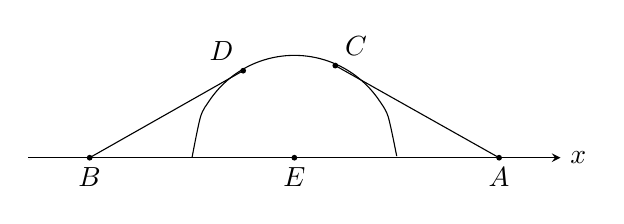
\begin{tikzpicture}[scale=1.3, >=stealth]
  \draw[->] (-2.6,0) -- (2.6,0) node[right] {$x$};
  \draw[domain=-1:1, smooth] plot ({\x},{sqrt(1-\x*\x)});
  \draw (-2,0) -- (-0.5,0.85);
  \draw (2,0) -- (0.4,0.9);
  \fill (0,0) circle (0.8pt) node[below] {$E$};
  \fill (-2,0) circle (0.8pt) node[below] {$B$};
  \fill (2,0) circle (0.8pt) node[below] {$A$};
  \fill (-0.5,0.85) circle (0.8pt) node[above left] {$D$};
  \fill (0.4,0.9) circle (0.8pt) node[above right] {$C$};
  \draw (-1,0) -- (1,0);
\end{tikzpicture}
\end{center}

題意の体積を$V(a)$とする。$B,D,C,A$の順に，$B$を頂点とする円錐，$D,C$間の弧を回転させた部分，$A$を頂点とする円錐に分けて，
\[
V(a)=\triangle_D+\bigcirc_C^D+\triangle_C \quad\cdots\text{③}
\]
であり，
\[
\triangle_D=\frac13\cdot(\pi\sin^2\beta)\cdot(a-\cos\beta+2)
\]
\[
=\frac{\pi}{3}\left(1-\left(\frac{1}{2+a}\right)^2\right)\left(a+2-\frac{1}{2+a}\right)
\]
\[
=\frac{\pi}{3}\cdot\frac{\{(2+a)^2-1\}^2}{(2+a)^3}
\]
\[
\bigcirc_C^D=\pi\int_{a-\cos\beta}^{a+\cos\alpha}\{1-(x-a)^2\}dx
\]
\[
=\pi\int_{-\cos\beta}^{\cos\alpha}(1-x^2)dx
\]
\[
=\pi\left[x-\frac13x^3\right]_{-\frac{1}{2+a}}^{\frac{1}{2-a}} \quad(\because②)
\]
\[
=\pi\left\{\left(\frac{1}{2-a}+\frac{1}{2+a}\right)-\frac13\left(\left(\frac{1}{2-a}\right)^3+\left(\frac{1}{2+a}\right)^3\right)\right\}
\]
\[
\triangle_C=\frac13(\pi\sin^2\alpha)(2-a-\cos\alpha)
\]
\[
=\frac{\pi}{3}\left(1-\left(\frac{1}{2-a}\right)^2\right)\left(2-a-\frac{1}{2-a}\right)
\]
\[
=\frac{\pi}{3}\cdot\frac{\{(2-a)^2-1\}^2}{(2-a)^3}
\]
を③に代入して，
\[
V(a)=\frac{\pi}{3}\left[\frac{\{(2-a)^2-1\}^2}{(2-a)^3}+\frac{\{(2+a)^2-1\}^2}{(2+a)^3}-\frac{1}{(2-a)^3}-\frac{1}{(2+a)^3}\right]+\pi\left[\frac{1}{2+a}+\frac{1}{2-a}\right]
\]
\[
=\frac{\pi}{3}\left[\frac{(a+3)^2(a^2+4a+2)}{(2+a)^3}+\frac{(a-3)^2(a^2-4a+2)}{(2-a)^3}\right]+\pi\left[\frac{1}{2+a}+\frac{1}{2-a}\right]
\]
\[
=\frac{\pi}{3}\left[\frac{a^3+4a+2+3}{2+a}+\frac{a^3-4a+2+3}{2-a}\right]
\]
\[
=\frac{\pi}{3}\left[a+2+\frac{1}{2+a}+2-a+\frac{1}{2-a}\right]
\]
\[
=\frac{\pi}{3}\left(4+\frac{1}{2+a}+\frac{1}{2-a}\right)
\]
\end{proof}

\newpage

\section*{第4問}

\begin{proof}[解]
$f(x)=x^3+ax^2+(b-a-1)x$

\textbf{(1)} $f'(x)=3x^2+2ax+(b-a-1)$だから，これが$x\ge0$で0以上であるような$(a,b)$を求めれば良い（$a,b\in\mathbb{R}$）。軸$x=-\dfrac13a$で場合分け。

\textbf{$1^\circ$ $-\dfrac13a\le0\ \therefore\ a\ge0$の時}

条件は$f'(0)\ge0\iff b\ge a+1$

\textbf{$2^\circ$ $0\le-\dfrac13a\ \therefore\ a\le0$の時}

条件は$f'(-\tfrac13a)\ge0\iff b\ge\dfrac13a^2+a+1$

以上をまとめ，図示して下図斜線部
\[
\begin{cases}
a\le0\text{の時}\ b\ge\dfrac13a^2+a+1 \\
a\ge0\text{の時}\ b\ge a+1
\end{cases}
\]

\begin{center}
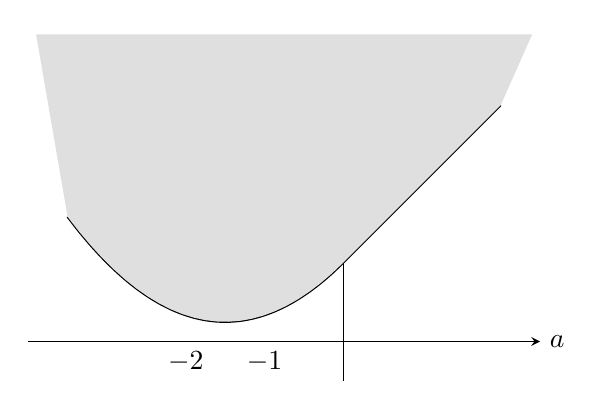
\begin{tikzpicture}[scale=1.0, >=stealth]
  \draw[->] (-4,0) -- (2.5,0) node[right] {$a$};
  \draw[->] (0,-0.5) -- (0,3.5) node[above] {$b$};
  \draw[domain=-3.5:0, smooth, thick] plot (\x,{\x*\x/3+\x+1});
  \draw[domain=0:2, smooth, thick] plot (\x,{\x+1});
  \fill[gray!25, domain=-3.5:0, variable=\x] plot ({\x},{\x*\x/3+\x+1}) -- (0,3.9) -- (-3.9,3.9) -- cycle;
  \fill[gray!25, domain=0:2, variable=\x] plot ({\x},{\x+1}) -- (2.4,3.9) -- (0,3.9) -- cycle;
  \node[below] at (-2,0) {$-2$};
  \node[below] at (-1,0) {$-1$};
\end{tikzpicture}
\end{center}

\textbf{(2)} $(a,b)$が$G$をうごく時，$0\le x$で$f(x)$は単調増加かつ$f(1)=b$から，グラフの概形は右図で，斜線部が求める面積$K$に等しい。したがって，与式$S$として
\[
S=b-\int_0^1f(x)dx
\]
\[
=b-\left(\frac14+\frac13a+\frac12(b-a-1)\right)
\]
\[
=\frac12b+\frac16a+\frac14 \quad\cdots\text{①}
\]
である。$a$を固定すると，①から，

\textbf{$a\le0$の時}
\[
\min S=\frac16a+\frac12\left(\frac13a^2+a+1\right)+\frac14
\]
\[
=\frac16a^2+\frac23a+\frac34
\]
\[
=\frac16(a+2)^2+\frac1{12}\ge\frac1{12} \quad(\text{等号成立は}a=-2)
\]

\textbf{$a\ge0$の時}
\[
\min S=\frac16a+\frac12(a+1)+\frac14
\]
\[
=\frac23a+\frac34\ge\frac34 \quad(\because a=0)
\]

だから，$\min S=\dfrac1{12}$
\end{proof}

\newpage

\section*{第5問}

\begin{proof}[解]
$f(x)=x^3-ax^2+bx-c$とおく。$f(x)=0$が整数解$x=k$を持つ時，
\[
c=k(k^2-ak+b) \quad\cdots\text{①}
\]
$k<0$の時，$k^2-ak+b>0$だから不適。$c=1,2,\cdots,6$だから下表をうる（複号同順）。ただし，$k<0$の時，$k^2-ak+b>0$から不適。
\begin{center}
\begin{tabular}{c|l}
$c$ & $(k,k^2-ak+b)$ \\
\hline
1 & $(1,1)$ \\
2 & $(2,1)$，$(1,2)$ \\
3 & $(3,1)$，$(1,3)$ \\
4 & $(4,1)$，$(2,2)$，$(1,4)$ \\
5 & $(5,1)$，$(1,5)$ \\
6 & $(6,1)$，$(3,2)$，$(2,3)$，$(1,6)$
\end{tabular}
\end{center}
①の時，$a=b$ $\therefore\ (a,b)=(1,1),(2,2),(3,3),(4,4),(5,5),(6,6)$

②　$-2a+b=-3$ $(a,b)=(2,1),(3,3),(4,5)$

③　$-a+b=1$ $(a,b)=(1,2),(2,3),(3,4),(4,5),(5,6)$

④　$-3a+b=-8$ $(a,b)=(3,1),(4,4)$

⑤　$-a+b=2$ $(a,b)=(1,3),(2,4),(3,5),(4,6)$

⑥　$-4a+b=-15$ $(a,b)=(4,1),(5,5)$

⑦　$-2a+b=-2$ $(a,b)=(2,2),(3,4),(4,6)$

⑧　$-a+b=3$ $(a,b)=(1,4),(2,5),(3,6)$

⑨　$-5a+b=-24$ $(a,b)=(5,1),(6,6)$

⑩　$-a+b=4$ $(a,b)=(1,5),(2,6)$

⑪　$-6a+b=-35$ $(a,b)=(6,1)$

⑫　$-3a+b=-7$ $(a,b)=(3,2),(4,5)$

⑬　$-2a+b=-1$ $(a,b)=(1,1),(2,3),(3,5)$

⑭　$-a+b=5$ $(a,b)=(1,6)$

したがって，重複する$(a,b,c)=(4,5,2)$を1通りとして数えると，あわせて38通りだから，
\[
\frac{38}{6^3}=\frac{19}{108}
\]
\end{proof}

\end{document}
